\documentclass{article} % For LaTeX2e
\usepackage{nips14submit_e,times}
\usepackage{amsmath}
\usepackage{amsthm}
\usepackage{amssymb}
\usepackage{mathtools}
\usepackage{hyperref}
\usepackage{url}
\usepackage{algorithm}
\usepackage[noend]{algpseudocode}
%\documentstyle[nips14submit_09,times,art10]{article} % For LaTeX 2.09

\usepackage{graphicx}
\usepackage{caption}
\usepackage{subcaption}

\def\eQb#1\eQe{\begin{eqnarray*}#1\end{eqnarray*}}
\def\eQnb#1\eQne{\begin{eqnarray}#1\end{eqnarray}}
\providecommand{\e}[1]{\ensuremath{\times 10^{#1}}}
\providecommand{\pb}[0]{\pagebreak}
\DeclarePairedDelimiter\ceil{\lceil}{\rceil}
\DeclarePairedDelimiter\floor{\lfloor}{\rfloor}

\newcommand{\E}{\mathrm{E}}
\newcommand{\Var}{\mathrm{Var}}
\newcommand{\Cov}{\mathrm{Cov}}

\def\Qb#1\Qe{\begin{question}#1\end{question}}
\def\Sb#1\Se{\begin{solution}#1\end{solution}}

\newenvironment{claim}[1]{\par\noindent\underline{Claim:}\space#1}{}
\newtheoremstyle{quest}{\topsep}{\topsep}{}{}{\bfseries}{}{ }{\thmname{#1}\thmnote{ #3}.}
\theoremstyle{quest}
\newtheorem*{definition}{Definition}
\newtheorem*{theorem}{Theorem}
\newtheorem*{lemma}{Lemma}
\newtheorem*{question}{Question}
\newtheorem*{preposition}{Preposition}
\newtheorem*{exercise}{Exercise}
\newtheorem*{challengeproblem}{Challenge Problem}
\newtheorem*{solution}{Solution}
\newtheorem*{remark}{Remark}
\usepackage{verbatimbox}
\usepackage{listings}
\usepackage{mathrsfs}
\title{DiffGeoI: \\
Problem Set I}


\author{
Youngduck Choi \\
CIMS \\
New York University\\
\texttt{yc1104@nyu.edu} \\
}


% The \author macro works with any number of authors. There are two commands
% used to separate the names and addresses of multiple authors: \And and \AND.
%
% Using \And between authors leaves it to \LaTeX{} to determine where to break
% the lines. Using \AND forces a linebreak at that point. So, if \LaTeX{}
% puts 3 of 4 authors names on the first line, and the last on the second
% line, try using \AND instead of \And before the third author name.

\newcommand{\fix}{\marginpar{FIX}}
\newcommand{\new}{\marginpar{NEW}}

\nipsfinalcopy % Uncomment for camera-ready version

\begin{document}


\maketitle

\begin{abstract}
This work contains solutions to the exercises of the problem set I.
\end{abstract}

\bigskip

\begin{question}[1]
\hfill
\begin{figure}[h!]
  \centering
    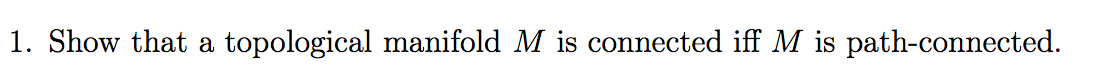
\includegraphics[width=0.7\textwidth]{DG-e1-p1.png}
\end{figure}
\end{question}
\begin{solution} \hfill \\
For any topological space, path-connected implies connected. We prove the converse.
Suppose $X$ is connected. Let $x \in X$, and set
\eQb
U &=& \{ y \in X \>|\> \text{ there is a path bewteen}\> x \>\text{and}\> y\}.
\eQe
Observe that $x \in U$ so $U$ is non-empty. Now, as $X$ is connected,
if $U$ and $U^c$ are both open, then $U^c$ is empty, and $U = X$, so
$X$ is path-connected. We show that $U$ is open. Let $y \in U$. Then,
there exists an open nbd of $y$, $O$, such that $O$ is homeomorphic to 
an open ball in $R^n$(this is equivalent to the locally euclidean
condition of topological manifold). Since
path-connectedness is preserved through homeomorphism, we conclude that $O$
is path connected and $O \subset U$. Therefore, $U$ is open and similarly
$U^c$ is open, and we are done. \hfill $\qed$ 

\end{solution}

\newpage

\begin{question}[2]
\hfill
\begin{figure}[h!]
  \centering
    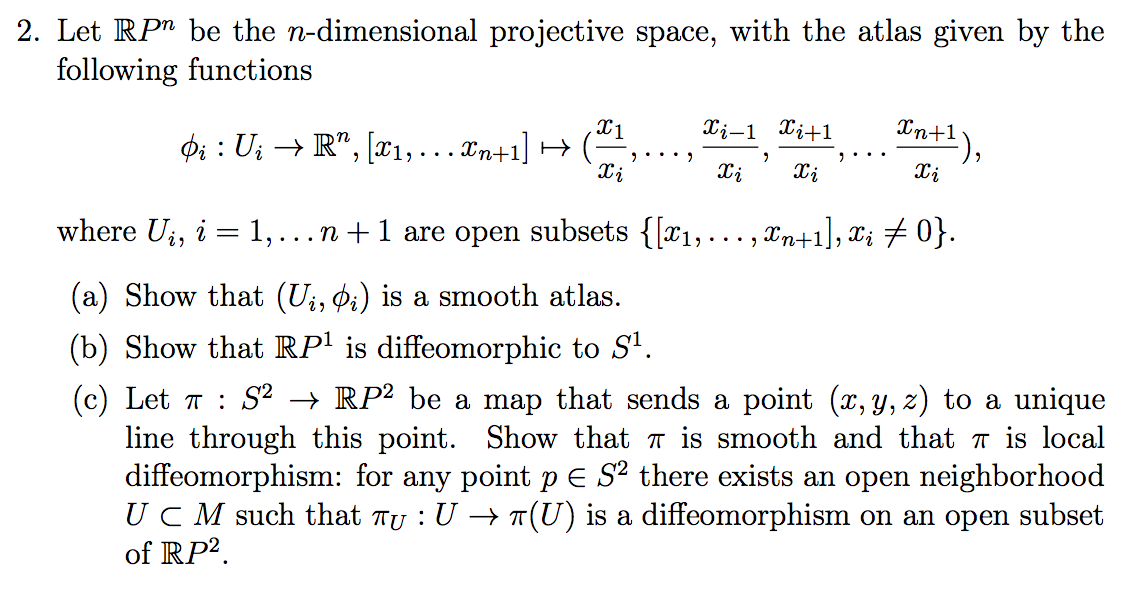
\includegraphics[width=0.7\textwidth]{DG-e1-p2.png}
\end{figure}
\end{question}
\begin{solution} \hfill \\
\textbf{(a)} Let $1 \leq i < j \leq n$. By symmetry, it suffices to show that
\eQb
\phi_j \circ \phi_i^{-1} : \phi_i(U_i \cap U_j) \to \phi_{j}(U_i \cap U_j) 
\eQe
is smooth. For any $a = (\dfrac{x_1}{x_i},...,\dfrac{x_{i+1}}{x_i},...,
\dfrac{x_{n+1}}{x_i}) \in \phi_i(U_i \cap U_j)$ with $x_i , x_j \neq 0$, 
\eQb
a \mapsto_{\phi_i^{-1}} [x_1,...,x_{n+1}] \mapsto_{\phi_j} (\dfrac{x_1}{
x_j},...,\dfrac{x_{j-1}}{x_j},\dfrac{x_{j+1}}{x_j},...,\dfrac{x_{n+1}}{x_i}).
\eQe
Since each coordinate map is smooth, we see that the transition map is smooth
and since the indices were arbitrary, the atlas is smooth. \hfill $\qed$

\bigskip

\textbf{(b)} Here, we choose to work with the stereographic projection chart on
$S^1$. Consider the map $\pi:S^1 \to \mathbb{R}P1$ defined by
\eQb
(x,y) &\mapsto& [1-y:x]
\eQe
for $(x,y) \in S^1$ such that $y \neq 1$, and
\eQb
(x,y) &\mapsto& [0:1]
\eQe
for $(x,y) \in S^1$ such that $y = 1$. Now, in chosen coordinates
\eQb
\pi_{1,1}(p) = p \\
\pi_{2,1}(p) = \dfrac{1}{p} \\
\pi_{1,2}(p) = \dfrac{1}{p} \\
\pi_{2,2}(p) = p \\.
\eQe
(This result is well-known; we show a more detailed computation in part c.)
Hence, all coordinate expressions are smooth, so $\pi$ is smooth. $\pi$
is one-to-one and in local charts the inverses are smooth as well. Hence,
we see that $\pi$ is a diffeomorphism. \hfill $\qed$ 

\bigskip

\textbf{(c)} 
We choose the smooth structure of $S^2$ to be the one
that contains the projection charts.
Let $p = (x^*,y^*,z^*) \in S^2$ and assume without loss of generality that
$z^* > 0$. Choose a chart $(U_z^+, \psi_z)$ of $p$ where 
\eQb
U_{z^+} &=& \{ p = (x,y,z) \in S^2 \> :\> z > 0 \} 
\eQe 
with $\psi_z: U_{z^+} \to \mathbb{R}^2$ defined by
\eQb
p = (x,y,z) \in U_{z^+} \mapsto (x,y). 
\eQe
Now, observe that with $z^* > 0$, $\pi(z^*) \in U_3$, so we can choose 
$(U_3,\phi_3)$
for a chart at $\pi(z^*)$. We now claim that
\eQb
\phi_3 \circ  \pi \circ \psi_z^{-1}:\psi_z(U_z^+) \to U_3 
\eQe
is smooth at $\psi(p)$. For each $(x,y) \in \psi(U_z^{+})$, we have
\eQb
(x,y) &\mapsto_{\psi_{z}^{-1}}& (x,y,(1-x^2-y^2)^{\frac{1}{2}})
\mapsto_{\pi} [x,y,(1-x^2-y^2)^{\frac{1}{2}}] \\
&\mapsto_{\phi_3}& 
(\dfrac{x}{(1-x^2-y^2)^{\frac{1}{2}}},\dfrac{y}{(1-x^2-y^2)^{\frac{1}{2}}}) 
\eQe
which simplifies to
\eQb
(x,y) \mapsto_{\phi_3 \circ \pi \circ \psi_{z}^{-1}} (\dfrac{x}{(1-x^2-y^2)^{
\frac{1}{2}}},
\dfrac{y}{(1-x^2-y^2)^{\frac{1}{2}}}).
\eQe
Therefore, we see that each component is smooth, and $\phi^3 \circ \pi 
\circ \psi_{z}^{-1}$ is smooth, so $\pi$ is smooth.

\bigskip
 
Now, it is easy to see that $\pi$ in fact gives the diffeomorphism as claimed.
By symmetry, on any chart, $\pi$ is a bijection from $U$ to $\pi(U)$, as we have 
eliminated the $2-1$ mapping by only considering positive or negative parts
in all dimensions. It is also true that $\pi(U)$ is open. Restricted
to $\pi(U)$ by the same computation as above, $\pi^{-1}$ is smooth, so we see
that $\pi$ is a local diffeomorphism. Formally, fix $p \in S^2$. Choose a chart
that contains $p$, $U$, then, $\pi$ restircted to $U$ gives a diffeomorphism
as required. \hfill $\qed$ 

\end{solution}

\newpage

\begin{question}[3]
\hfill
\begin{figure}[h!]
  \centering
    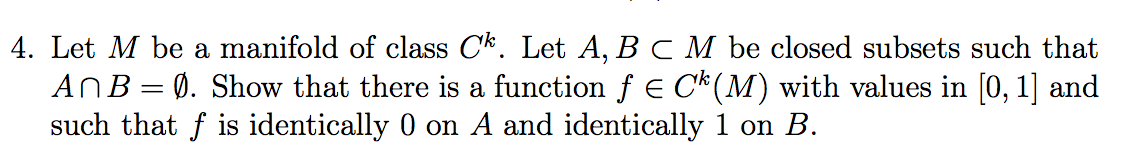
\includegraphics[width=0.7\textwidth]{DG-e1-p3.png}
\end{figure}
\end{question}
\begin{solution} \hfill \\
Without loss of generality, we assume smooth structure on $M$ and prove that a smooth
map with the desired property exists.
One should remark that this version of smooth urysohn's lemma is easier to prove than
the version on the normal space that is merely continuous, 
as we have more structure from the smooth manifold assumption. It is sufficient to
prove that for any open set $O$ there exists a smooth $f:M \to [0,\infty)$ such that
$f^{-1}(0) = (M\setminus O)$. First suppose that $O$ is a product of open intervals
in some $\mathbb{R}^n$. Then, there exists a bump function, positive on $O$ and
vanishes on the complement. Now, for $O$ open in $\mathbb{R}^n$, write it
as a union of open cubes such that for any point in $O$, there is
finitely many open cubes that cover it. Sum of the bump functions from the previous
result gives the desired construction. Now, consider an open set that has 
a chart defined on it. Then, by pull-back and using the previous result, we obtain
the desired function. Again, for the general open set, use the locally finite 
cover of charts and sum then constructed functions. 

\bigskip

Now let $C_1, C_2$ be closed subsets of $M$ such that $C_1 \cap C_2 = \empty$.
Choose $f_1$ and $f_2$ smooth functions on $M$ such that $f_1^{-1}(0) = C_1$
and $f_2^{-1}(0) = C_2$. Set 
\eQb
f &=& \dfrac{f_1}{f_1 + f_2}.
\eQe  
It follows that $f$ is the desired function. \hfill $\qed$ 
\end{solution}

\end{document}
